\documentclass[12pt]{article}
\usepackage[utf8]{inputenc}
\usepackage[T2A]{fontenc}
\usepackage[russian]{babel}
\usepackage{amsmath, amssymb, amsfonts}
\usepackage{geometry}
\usepackage{multirow}
\usepackage{array}
\usepackage{graphicx, changepage}
\usepackage{pdflscape}
\usepackage{listings}
\usepackage{xcolor}
\usepackage{hyperref}
\usepackage[font=small,labelfont=bf]{caption}
\usepackage{csvsimple}

\geometry{a4paper, margin=2.5cm}
\graphicspath{ {../img/} }

\author{Лазар Владислав Игоревич, 416 группа}
\title{Отчёт по практическому заданию по ДГСП}

\hypersetup{
    colorlinks=true,
    linkcolor=black,
    filecolor=magenta,
    urlcolor=cyan,
}


\begin{document}
\maketitle

\newpage

\tableofcontents

\newpage

\section{Теоретическая часть}

\subsection{Исследуемое явление}

В данной работе рассматривается задача наблюдения за перемещающейся по плоскости тележкой. Состоянием тележки является её положение на плоскости (x, y, ориентация в пространстве) и угол поворота колёс. На плоскости в начале координат установлен локатор, измеряющий расстояние до тележки и угол направления на неё.
\newline

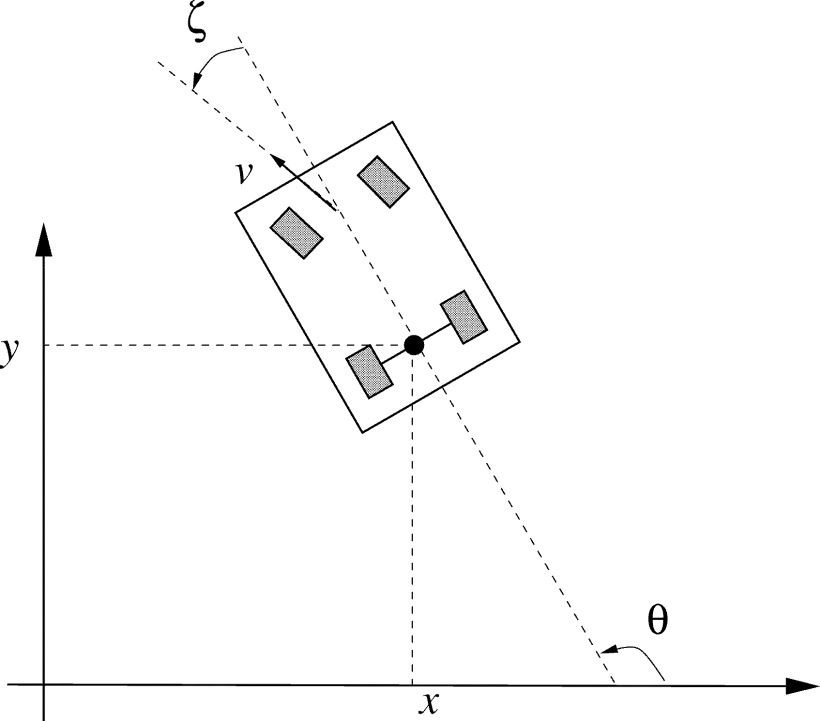
\includegraphics[width=1.0\linewidth]{../system.png}

\newpage

Далее будет описана используемая матемаическая модель. Типичная траектория получаемая с её помощью выглядит следующим образом:

\includegraphics[width=1.0\linewidth]{traj.png}

\subsection{Система наблюдения}

Математическая модель описывается системой с дискретным временем:

\begin{equation*}
	\begin{cases}
		x_{1, k} = x_{1, k-1} + T cos(\theta_{k-1}) cos(\phi_{k-1}) u_{1, k-1}           \\
		x_{2, k} = x_{2, k-1} + T sin(\theta_{k-1}) cos(\phi_{k-1}) u_{1, k-1}           \\
		\theta_k = \theta_{k-1} + T sin(\phi_{k-1}) \frac{u_{1, k-1}}{l} + \omega_{3, k} \\
		\phi_k = \phi_{k-1} + T u_{2, k-1} + \omega_{4, k}
	\end{cases}
\end{equation*}

где

\begin{itemize}
	\item $x_1$ - координата объекта по оси x
	\item $x_2$ - координата объекта по оси y
	\item $\theta$ - угол между направлением движения тележки и положительной полуосью Ox (ориентация на плоскости)
	\item $\phi$ - угол поворота колёс тележки относительно направления движения
	\item $T$ - параметр дискретизации системы по времени
	\item $l$ - расстояние между осями тележки
	\item $\omega$ - шум в модели динамики, $\omega_k \sim \mathcal{N}(0, Q)$
	\item $u_1$ - управляемая линейная скорость
	\item $u_2$ - управляемая угловая скорость
\end{itemize}

Наблюдения определяются следующим образом:

\begin{equation*}
	\begin{cases}
		r_k = \sqrt{x_{1, k}^2 + x_{2, k}^2} + \nu_{1, k} \\
		\alpha_k = \arctan(\frac{x_{2, k}}{x_{1, k}}) + \nu_{2, k}
	\end{cases}
\end{equation*}

где

\begin{itemize}
	\item $r_k$ - расстояние от локатора до цели
	\item $\alpha_k$ - угол направления от локатора к цели
	\item $\nu$ - шум в наблюдениях, $\nu \sim \mathcal{N}(0, R)$
\end{itemize}

\newpage

\section{Практическая часть}

\subsection{Значения параметров системы}

В численных экспериментах установим следующие параметры системы:

\[
	l=0.1, \; u_1 = 3, \; u_2 = 0
\]

Шаги по времени:

\[
	\delta_1 = \delta_2 = 10^{-3}, \; \delta_1 = 10^{-2}, \; T_{max} = 1
\]

Заметим, что равенство $\delta_1$ и $\delta_2$ следует из того, что система заране дискретизирована.

Также для наблюдений вместо $\arctan$ возьмём $\arctan_2$. Это обусловлено тем, что область действия $\arctan$ - $[- \frac{\pi}{2}; \frac{\pi}{2} ]$, а $\arctan_2$ - весь тригонометрический круг. Благодаря этому мы сможем избежать ошибки наблюдений с неправильным определением полуплоскости.

Матрицы шумов возьмём следующими:

\[
	Q = \begin{bmatrix}
		3 \cdot 10^{-7} & 0                & 0                & 0                \\
		0               & 3 \cdot 10 ^{-7} & 0                & 0                \\
		0               & 0                & 3 \cdot 10 ^{-5} & 0                \\
		0               & 0                & 0                & 3 \cdot 10 ^{-5} \\
	\end{bmatrix}
\]

\[
	R = 5 \cdot 10^{-3} \cdot I_2
\]

Начальное значение траектории моделируется следующим образом:

\[
	X_0 \sim \mathcal{N}(0, 0.3 \cdot I_4)
\]

Все необходимые для фильтрации параметры были посчитаны аналитически во время работы программы с помощью соответствующих пакетов Python (filterpy, sympy). Реализации всех фильтров также взяты из соответствующих пакетов на Python. Также для достижения большей точности были использованы 128-битные числа с плавающей точкой (стандарт IEEE 754).

\subsection{Сравнение работы алгоритмов}


\begin{landscape}
	\subsubsection{Оценки траектории}
	\captionof{figure}{Оценка $x_1$}
	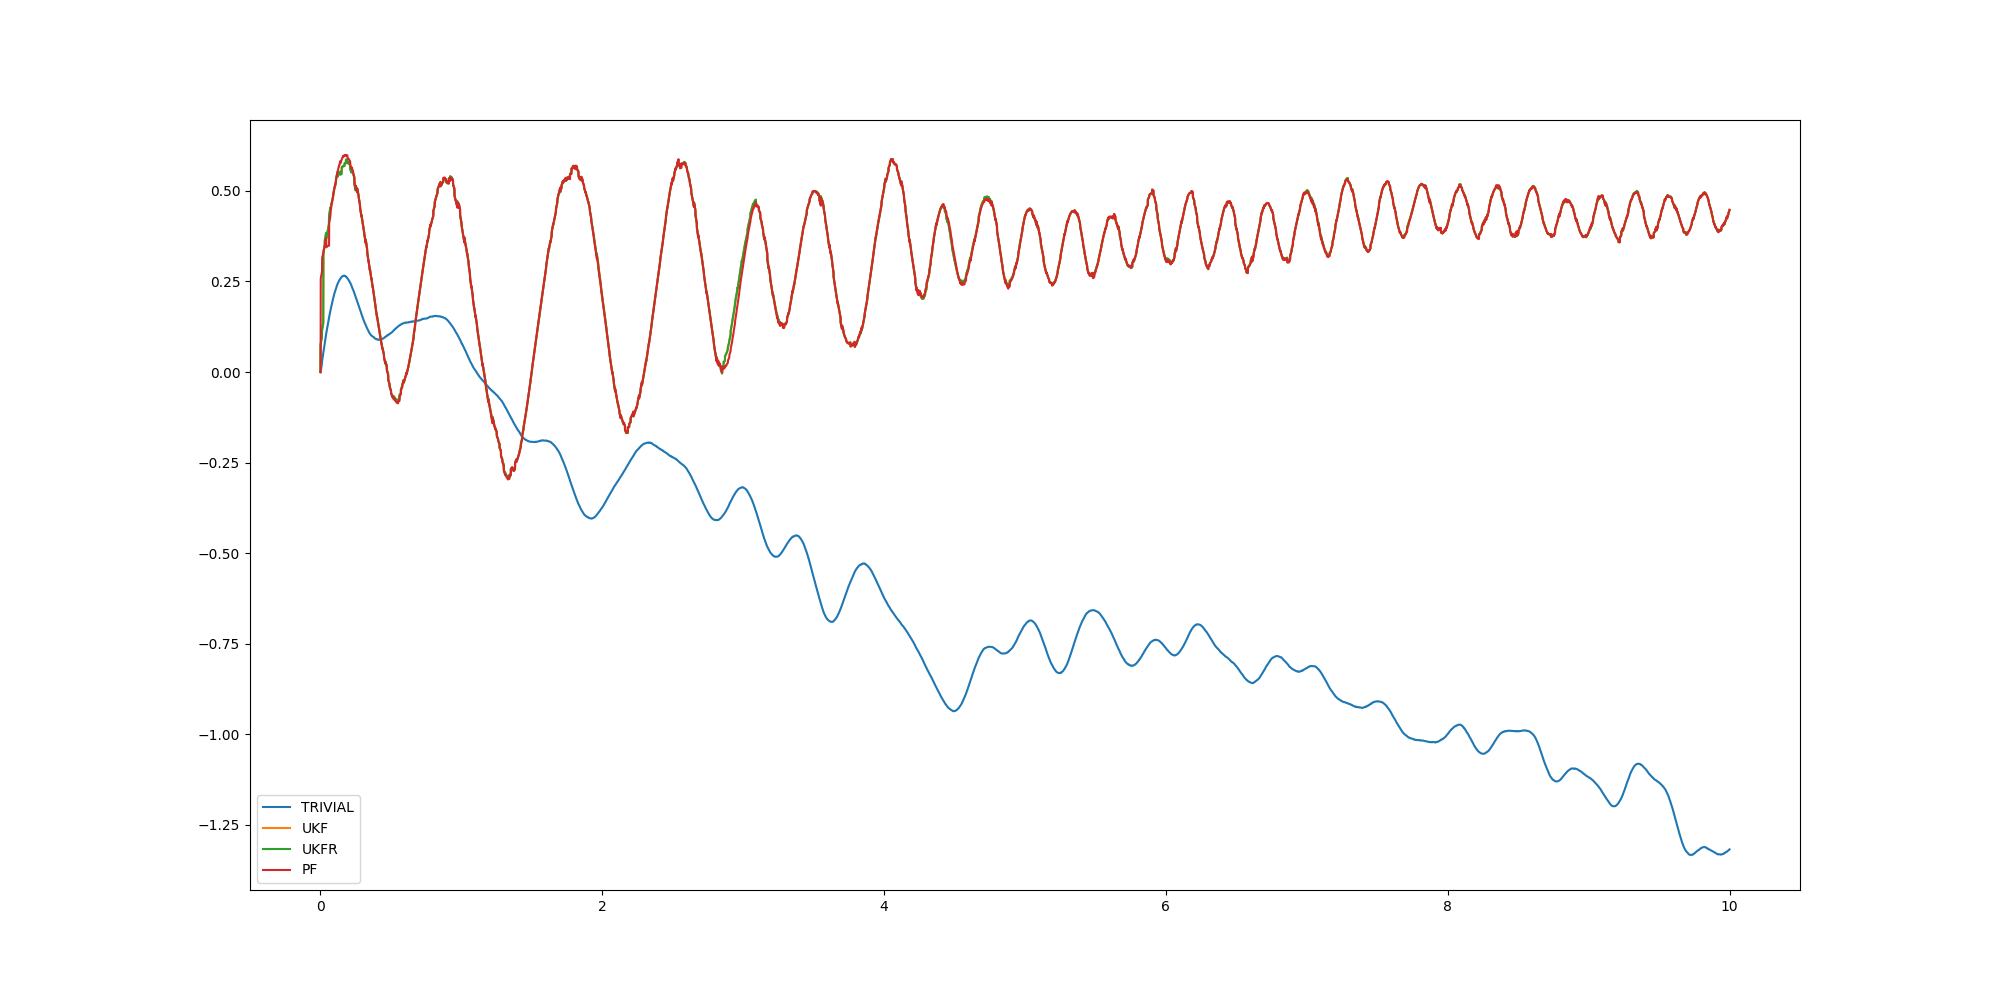
\includegraphics[width=1.0\linewidth]{example/estimate_0.png}\newpage
\end{landscape}

\begin{landscape}
	\captionof{figure}{Оценка $x_2$}
	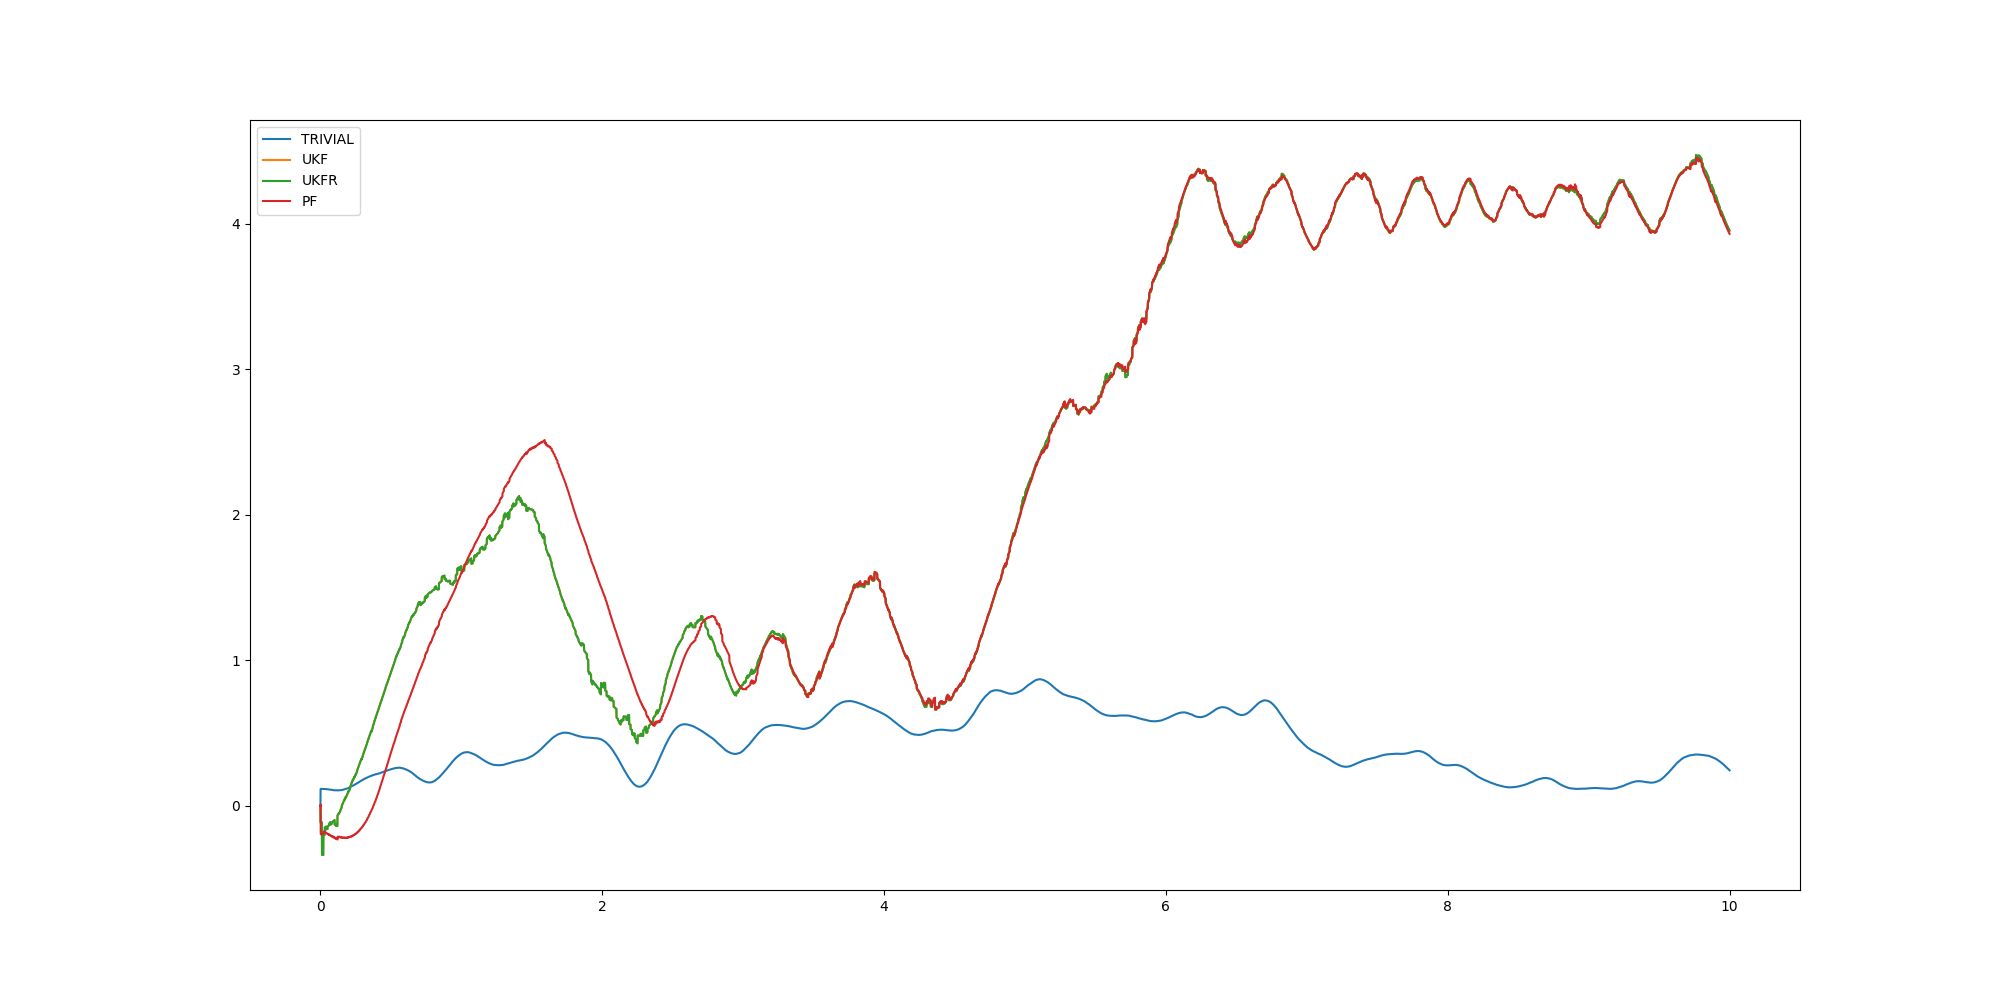
\includegraphics[width=1.0\linewidth]{example/estimate_1.png}\newpage
\end{landscape}

\begin{landscape}
	\captionof{figure}{Оценка $\theta$}
	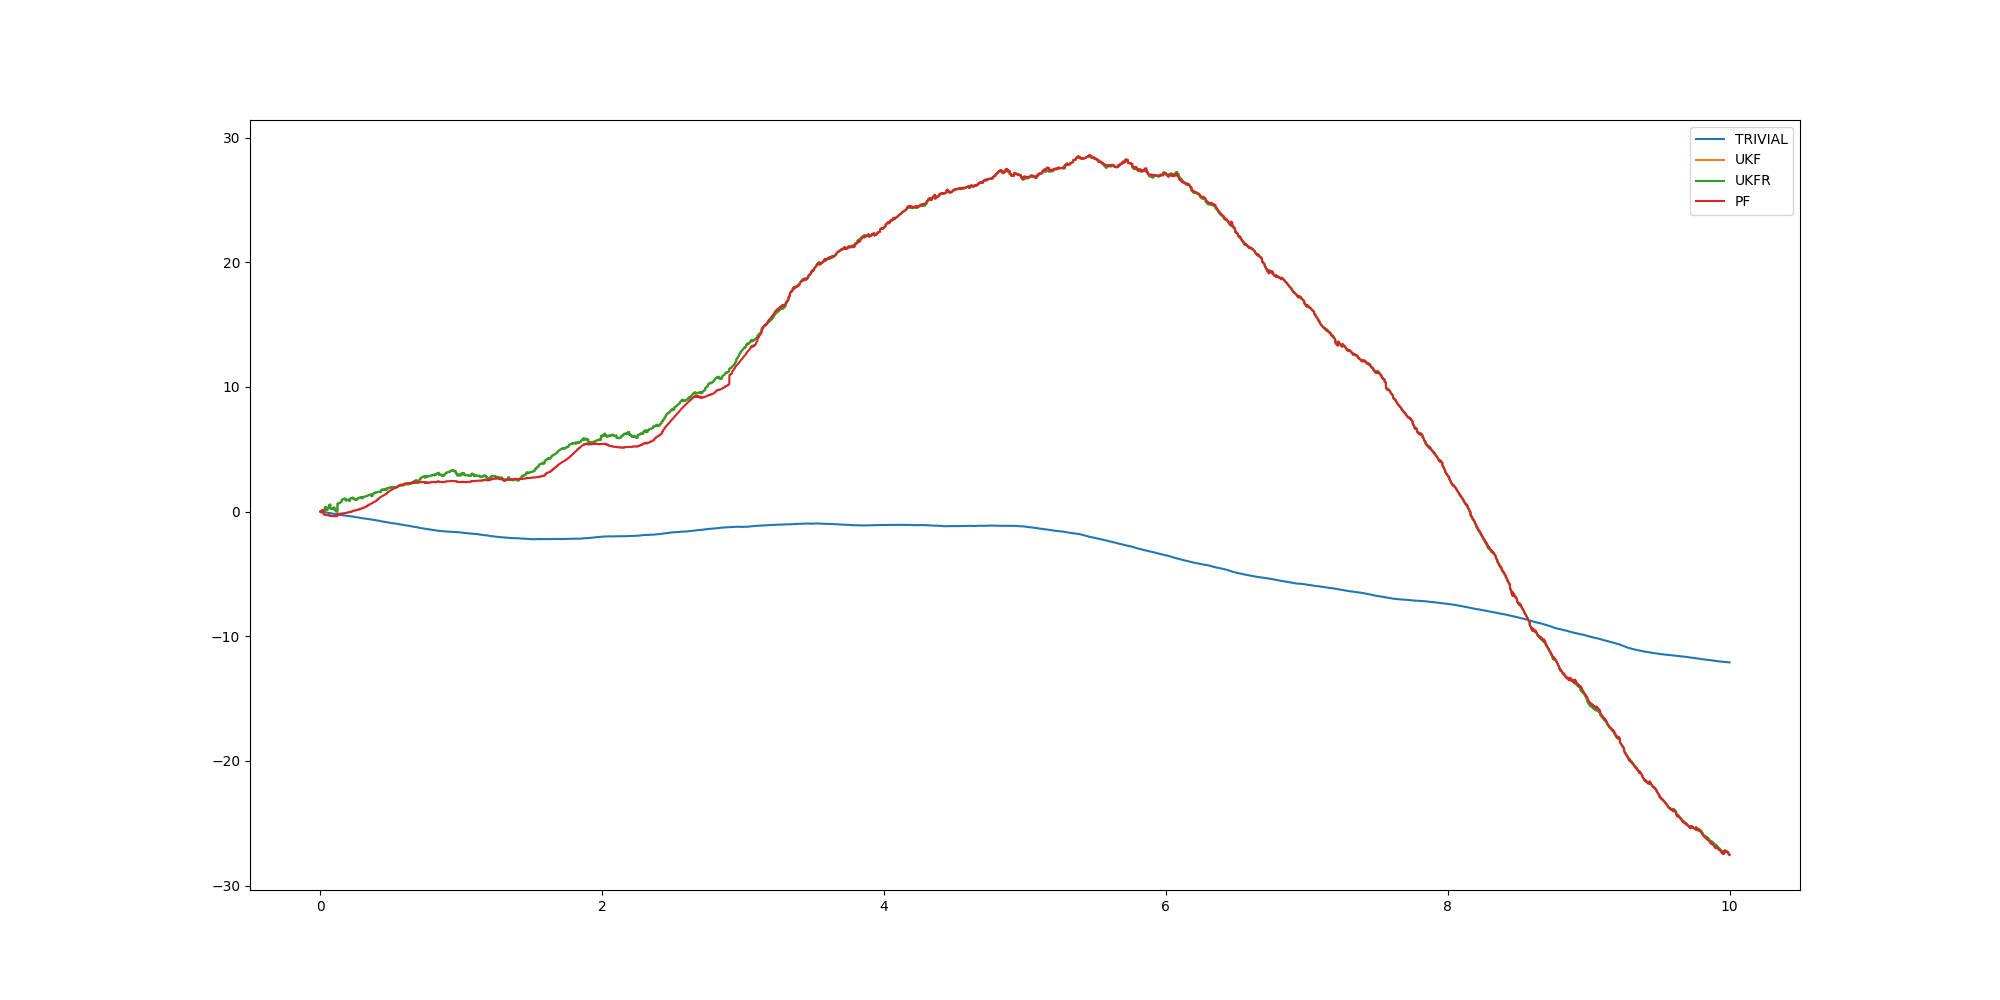
\includegraphics[width=1.0\linewidth]{example/estimate_2.png}\newpage
\end{landscape}

\begin{landscape}
	\captionof{figure}{Оценка $\phi$}
	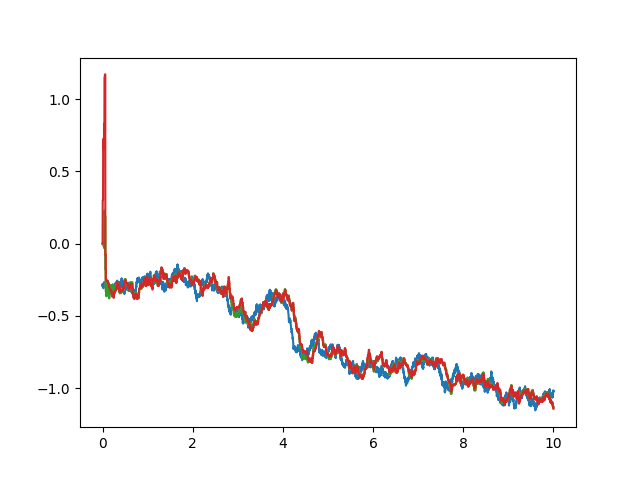
\includegraphics[width=1.0\linewidth]{example/estimate_3.png}\newpage
\end{landscape}

\newpage

\begin{landscape}
	\subsubsection{Ошибки оценивания $x_1$}
	\includegraphics[width=1.0\linewidth]{example/err_0_trivial.png}\newpage
\end{landscape}

\begin{landscape}
	\includegraphics[width=1.0\linewidth]{example/err_0_ukf.png}\newpage
\end{landscape}

\begin{landscape}
	\includegraphics[width=1.0\linewidth]{example/err_0_ukfr.png}\newpage
\end{landscape}

\begin{landscape}
	\includegraphics[width=1.0\linewidth]{example/err_0_pf.png}\newpage
\end{landscape}

\begin{landscape}
	\subsubsection{Ошибки оценивания $x_2$}
	\includegraphics[width=1.0\linewidth]{example/err_1_trivial.png}\newpage
\end{landscape}

\begin{landscape}
	\includegraphics[width=1.0\linewidth]{example/err_1_ukf.png}\newpage
\end{landscape}

\begin{landscape}
	\includegraphics[width=1.0\linewidth]{example/err_1_ukfr.png}\newpage
\end{landscape}

\begin{landscape}
	\includegraphics[width=1.0\linewidth]{example/err_1_pf.png}\newpage
\end{landscape}

\begin{landscape}
	\subsubsection{Ошибки оценивания $\theta$}
	\includegraphics[width=1.0\linewidth]{example/err_2_trivial.png}\newpage
\end{landscape}

\begin{landscape}
	\includegraphics[width=1.0\linewidth]{example/err_2_ukf.png}\newpage
\end{landscape}

\begin{landscape}
	\includegraphics[width=1.0\linewidth]{example/err_2_ukfr.png}\newpage
\end{landscape}

\begin{landscape}
	\includegraphics[width=1.0\linewidth]{example/err_2_pf.png}\newpage
\end{landscape}

\begin{landscape}
	\subsubsection{Ошибки оценивания $\phi$}
	\includegraphics[width=1.0\linewidth]{example/err_3_trivial.png}\newpage
\end{landscape}

\begin{landscape}
	\includegraphics[width=1.0\linewidth]{example/err_3_ukf.png}\newpage
\end{landscape}

\begin{landscape}
	\includegraphics[width=1.0\linewidth]{example/err_3_ukfr.png}\newpage
\end{landscape}

\begin{landscape}
	\includegraphics[width=1.0\linewidth]{example/err_3_pf.png}\newpage
\end{landscape}

\begin{landscape}
	\subsubsection{Графики ошибок для нерасходящихся траекторий}
	\captionof{figure}{Ошибка $x_1$}
	\includegraphics[width=1.0\linewidth]{err/conv/0.png}\newpage
\end{landscape}

\begin{landscape}
	\captionof{figure}{Ошибка $x_2$}
	\includegraphics[width=1.0\linewidth]{err/conv/1.png}\newpage
\end{landscape}

\begin{landscape}
	\captionof{figure}{Ошибка $\theta$}
	\includegraphics[width=1.0\linewidth]{err/conv/2.png}\newpage
\end{landscape}

\begin{landscape}
	\captionof{figure}{Ошибка $\phi$}
	\includegraphics[width=1.0\linewidth]{err/conv/3.png}\newpage
\end{landscape}

\begin{landscape}
	\subsubsection{Графики ошибок для всех траекторий}
	\captionof{figure}{Ошибка $x_1$}
	\includegraphics[width=1.0\linewidth]{err/all/0.png}\newpage
\end{landscape}

\begin{landscape}
	\captionof{figure}{Ошибка $x_2$}
	\includegraphics[width=1.0\linewidth]{err/all/1.png}\newpage
\end{landscape}

\begin{landscape}
	\captionof{figure}{Ошибка $\theta$}
	\includegraphics[width=1.0\linewidth]{err/all/2.png}\newpage
\end{landscape}

\begin{landscape}
	\captionof{figure}{Ошибка $\phi$}
	\includegraphics[width=1.0\linewidth]{err/all/3.png}\newpage
\end{landscape}

\subsubsection{Численные результаты}

\begin{table*}[!ht]
	\centering
	\csvreader[
		tabular={|c|c|},
		table head = \hline \textbf{Метод} & \textbf{Процент расходящихся траекторий} \\ \hline,
		late after line= \\,
		late after last line=\\\hline
	]{../stats/diverge.csv}{estimator=\estimator,divergence=\divergence}
	{\estimator & \divergence}
\end{table*}

\begin{table*}[!ht]
	\centering
	\csvreader[
		tabular={|c|c|c|c|},
		table head = \hline \textbf{Время} & \textbf{UKF} & \textbf{UKFR} & \textbf{PF} \\ \hline,
		late after line= \\,
		late after last line=\\\hline
	]{../stats/error_0.csv}{t=\t,ukf=\ukf,ukfr=\ukfr,pf=\pf}
	{\t & \ukf & \ukfr & \pf}
	\centering
	\caption{Средние ошибки фильтров на оценивания $x_1$}
\end{table*}

\begin{table*}[!ht]
	\centering
	\csvreader[
		tabular={|c|c|c|c|},
		table head = \hline \textbf{Время} & \textbf{UKF} & \textbf{UKFR} & \textbf{PF} \\ \hline,
		late after line= \\,
		late after last line=\\\hline
	]{../stats/error_1.csv}{t=\t,ukf=\ukf,ukfr=\ukfr,pf=\pf}
	{\t & \ukf & \ukfr & \pf}
	\centering
	\caption{Средние ошибки фильтров оценивания $x_2$}
\end{table*}

\begin{table*}[!ht]
	\centering
	\csvreader[
		tabular={|c|c|c|c|},
		table head = \hline \textbf{Время} & \textbf{UKF} & \textbf{UKFR} & \textbf{PF} \\ \hline,
		late after line= \\,
		late after last line=\\\hline
	]{../stats/error_2.csv}{t=\t,ukf=\ukf,ukfr=\ukfr,pf=\pf}
	{\t & \ukf & \ukfr & \pf}
	\centering
	\caption{Средние ошибки фильтров оценивания $\theta$}
\end{table*}
\begin{table*}[!ht]
	\centering
	\csvreader[
		tabular={|c|c|c|c|},
		table head = \hline \textbf{Время} & \textbf{UKF} & \textbf{UKFR} & \textbf{PF} \\ \hline,
		late after line= \\,
		late after last line=\\\hline
	]{../stats/error_3.csv}{t=\t,ukf=\ukf,ukfr=\ukfr,pf=\pf}
	{\t & \ukf & \ukfr & \pf}
	\centering
	\caption{Средние ошибки фильтров оценивания $\phi$}
\end{table*}

\newpage

\section{Выводы по расчётам}

Из графиков видно, что оценки UKF и его корневой модификации ведут себя абсолютно одинаково. Это логично следует из вышеописанных особенностей реализации для 128-битных чисел. Более подробно о таком поведении фильтров Калмана написано в \href{https://filterpy.readthedocs.io/en/latest/kalman/SquareRootFilter.html}{соответствующем разделе документации}. \newline
Также можно заметить, что лучше всего фильтры справляются с оценкой местоположения тележки, а хуже всего - с углами $\theta$ и $\phi$. Этому есть логичное объяснение: в качестве наблюдений мы получаем полярные координаты тележки. Благодаря этому мы достаточно точно можем строить оценку для $x_1$ и $x_2$. В то же время, в наблюдениях никоим образом не участвуют углы, поэтому информацию о них мы получаем косвенно через перемещение тележки. Более того, поскольку угловая скорость $u_2$ при расчётах взята равной нулю, поведение $\phi$ описывается винеровским процессом с соответствующими параметрами. Из-за этого оценивать его сложнее всего, хотя и возможно из изменения $\theta$. Но, поскольку все наблюдения зашумлены, а при изменении состояния также добавляется шум, эффект накопления ошибки сильнее всего виден именно на этой компоненте состояния. Тем не менее, основную задачу можно признать выполненной - полученный алгоритм достаточно точно оценивает траекторию движения цели несмотря на помехи. Также из таблиц можно увидеть, что оценка, полученная фильтром частиц, часто оказывается хуже оценки UKF (ошибка большге примерно в 1.5-1.6 раза), но при этом процент расходящихся траекторий у PF сильно меньше (6 против почти 17). То есть, в данном случае большая вычислительная сложность оправдывается большей стабильностью. Если также посмотреть на графики средних ошибок на всех и на неразваливающихся траекториях, будет видно, что фильтр частиц ведёт себя и на тех и на других траекториях похожим образом, в то время как средняя ошибка сигма-точечного фильтра сильно зависит от типа траектории. \newline
Если взглянуть на графики средних ошибок на всех траекториях, можно также заметить, что средняя ошибка растёт. Это может быть связано с тем, что, начиная с некоторого момента, тележка может начать кружить вокруг некоторой точки из-за неуправляемого роста угла поворота. В такие моменты становится сложно предсказать траекторию, так как малое изменение местоположения тележки по сравнению с погрешностью наблюдений сильно сказывается на работе фильтра, и для него такое движение с точки зрения постановки задачи становится мало отличимым от броуновского. Возможно, такого поведения цели можно избежать путём изменения управления с константного на зависящее от времени.

\end{document}
